
\documentclass{beamer}

\usepackage[brazil]{babel}
\usepackage{beamerthemesplit}
\usepackage{graphics}
\usepackage{graphicx}
\usepackage{hyperref}
\usepackage{listings}
\usepackage{color}
\usepackage{xcolor}
\usepackage[utf8]{inputenc}



\definecolor{MyDarkBlue}{rgb}{0,0.08,0.45}
\definecolor{MyDarkRed}{rgb}{0.65,0,0}
\definecolor{MyDarkGreen}{rgb}{0,0.45,0}
\definecolor{MyDarkYellow}{cmyk}{0,0,0.85,0.2}



\mode<presentation>
{
% \usetheme{AnnArbor}
% \usetheme{Ilmenau}
% \usetheme{Antibes}
% \usetheme{JuanLesPins}
% \usetheme{Bergen}
% \usetheme{Luebeck}
% \usetheme{Berkeley}
% \usetheme{Madrid}
% \usetheme{Berlin}
% \usetheme{Malmoe}
% \usetheme{Boadilla}
% \usetheme{Marburg}
% \usetheme{boxes}
% \usetheme{Montpellier}
 \usetheme{CambridgeUS}
% \usetheme{PaloAlto}
% \usetheme{Copenhagen}
% \usetheme{Pittsburgh}
% \usetheme{Darmstadt}
% \usetheme{Rochester}
% \usetheme{default}
% \usetheme{Singapore}
% \usetheme{Dresden}
% \usetheme{Szeged}
% \usetheme{Frankfurt}
 %\usetheme{Warsaw}
% \usetheme{Goettingen}
% \usetheme{Hannover}




%    \usecolortheme{albatross}% - modre ramecky, jinak modre pozadi
%    \usecolortheme{beetle}% - namodrale ramecky, sede pozadi
%    \usecolortheme{beaver}% - namodrale ramecky, sede pozadi
%    \usecolortheme{crane}% - zlute ramecky, bile pozadi
%    \usecolortheme{sidebartab}% - namodrale ramecky, sede pozadi
%    \usecolortheme{wolverine}% - namodrale ramecky, sede pozadi
    \usecolortheme{default}%
%    \usecolortheme{dolphin}% - bile a sedomodre ramecky, podobne default, svetlejsi
%    \usecolortheme{dove}% - bile ramecky, skoro cernobile
%    \usecolortheme{fly}% - sede pozadi i ramecky, nadpisy bile
%    \usecolortheme{lily}% - skoro stejne jako default, jen bile ramecky nadpisu
%    \usecolortheme{orchid}% - stejne jako default?
%    \usecolortheme{rose}% - stejne jako default?
%    \usecolortheme{seagull}% - podobne dolphin, sede ramecky, bile pozadi
%    \usecolortheme{seahorse}% - podobne dolphin, sede ramecky, bile pozadi
%    \usecolortheme{whale}% - stejne jako default?

\setbeamertemplate{items}[ball]
\setbeamercolor{subitem projected}{bg=gray}
\setbeamercolor{item}{bg=white}
\setbeamercolor{item}{fg=gray}
\setbeamercolor{frametitle}{fg=gray}
\setbeamercolor{frametitle}{bg=white}
\setbeamercolor{title}{fg=gray}

\setbeamercovered{transparent}
}



\title[DonkeySurvey]{DonkeySurvey: \\Coleta de dados sobre compartilhamento de arquivos em redes P2P}


% - Use the \inst{?} command only if the authors have different
%   affiliation.
\author[]{Beraldo Leal, Tássia Camões e Vinicius Pinheiro}
%\author[Raphael Cóbe]{Raphael Mendes de O. Cóbe\inst{1} \\
%raphael@ccsa.ufrn.br}

% - Use the \inst command only if there are several affiliations.
% - Keep it simple, no one is interested in your street address.
\institute[IME/USP]
{
Instituto de Matemática e Estatística - IME\\
Universidade de São Paulo - USP
}

\date{}


% This is only inserted into the PDF information catalog. Can be left
% out.
\subject{Talks}

% If you have a file called "university-logo-filename.xxx", where xxx
% is a graphic format that can be processed by latex or pdflatex,
% resp., then you can add a logo as follows:

\pgfdeclareimage{usp-logo}{img/usp-logo}
\logo{\pgfuseimage{usp-logo}}



% Delete this, if you do not want the table of contents to pop up at
% the beginning of each subsection:
%\AtBeginSubsection[]
%\AtBeginSection[]
%{
%\begin{frame}<beamer>
%\frametitle{Agenda}
%\tableofcontents[currentsection]
%\end{frame}
%}

% If you wish to uncover everything in a step-wise fashion, uncomment
% the following command:



\newenvironment{changemargin}[2]{%
\begin{list}{}{%
\setlength{\leftmargin}{#1}%
\setlength{\rightmargin}{#2}%
\setlength{\listparindent}{\parindent}%
\setlength{\itemindent}{\parindent}%
\setlength{\parsep}{\parskip}%
}%
\item[]}{\end{list}}

%\beamerdefaultoverlayspecification{<+->}

\begin{document}

\begin{frame}
\titlepage
\end{frame}

%\begin{frame}[allowframebreaks]
%\frametitle{Agenda}
%\tableofcontents
%% You might wish to add the option [pausesections]
%\end{frame}


\section{Introdução}

\subsection{Overview}

\begin{frame}
  \frametitle{DonkeySurvey}
\hspace{0.25in}
\setbeamercolor{uppercol}{fg=white,bg=MyDarkYellow}
\setbeamercolor{lowercol}{fg=black,bg=white}
 \begin{itemize}
      \item Contexto
      \begin{itemize}
          \item Necessidade de manter o histórico de conexões e arquivos compartilhados
          \item Clientes P2P disponíveis não possuem tal funcionalidade
          \begin{itemize}
              \item Ferramentas analisadas: p2pdetect, ed2kstats, aMule, MLDonkey
            \end{itemize}
        \end{itemize}
      
      \item Estratégias
     \begin{itemize}
          \item Modificar núcleo do MLDonkey
          \item Desenvolver um plugin
          \item Aplicação independente
      \end{itemize}

 \end{itemize}
\end{frame}

\begin{frame}
  \frametitle{DonkeySurvey}
\hspace{0.25in}
\setbeamercolor{uppercol}{fg=white,bg=MyDarkYellow}
\setbeamercolor{lowercol}{fg=black,bg=white}
     \begin{itemize}
         \item Como engatilhar ações para coleta? 
         \item Comunicação síncrona 
         \begin{itemize}
             \item Via telnet
             \item Utilizando mldonkey-command
         \end{itemize}
         \item Comunicação assíncrona 
         \begin{itemize}
             \item Via GUI-protocol
          \end{itemize}
      \end{itemize}
\end{frame}


\begin{frame}
\begin{changemargin}{-2cm}{-2cm}
  \begin{figure}
    \includegraphics[width=360px]{img/DonkeySurvey.ps}
  \end{figure} 
\end{changemargin}
\end{frame}


\begin{frame}
  \frametitle{Atividades realizadas}
\hspace{0.25in}
\setbeamercolor{uppercol}{fg=white,bg=MyDarkYellow}
\setbeamercolor{lowercol}{fg=black,bg=white}
 \begin{itemize}
  \item Estudo sobre o estado da arte de mecanismos para coleta e armazenamento de dados em redes de compartilhamento de arquivos P2P.
  \item Imersão na ferramenta escolhida, MLdonkey.
  \item Analise das possíveis estratégias de desenvolvimento do DonkeySurvey;
  \item Patch para adicionar a opção file\_up\_completed\_cmd e file\_up\_started\_cmd;
  \item Implementação parcial do GUIProtocol (Connection Phase);
  \item Implementação do script para automatizar os testes de upload e donwload entre clientes;
  \item Implementação inicial da base de dados (mysql). 
 \end{itemize}
\end{frame}

\begin{frame}
\begin{changemargin}{-2cm}{-2cm}
  \begin{figure}
    \includegraphics[width=300px]{img/ammap_tor.ps}
  \end{figure} 
\end{changemargin}
\end{frame}

\end{document}
